\section{Data link layer}
The data link layer is implemented in the form of two classes. The DataLinkLayer
object is instantiated by the backbone and the Frame and Datagram objects are
instantiated by the DataLinkLayer and destructed by it when processed.

%\begin{figure}[htb]
%	\begin{center}
%	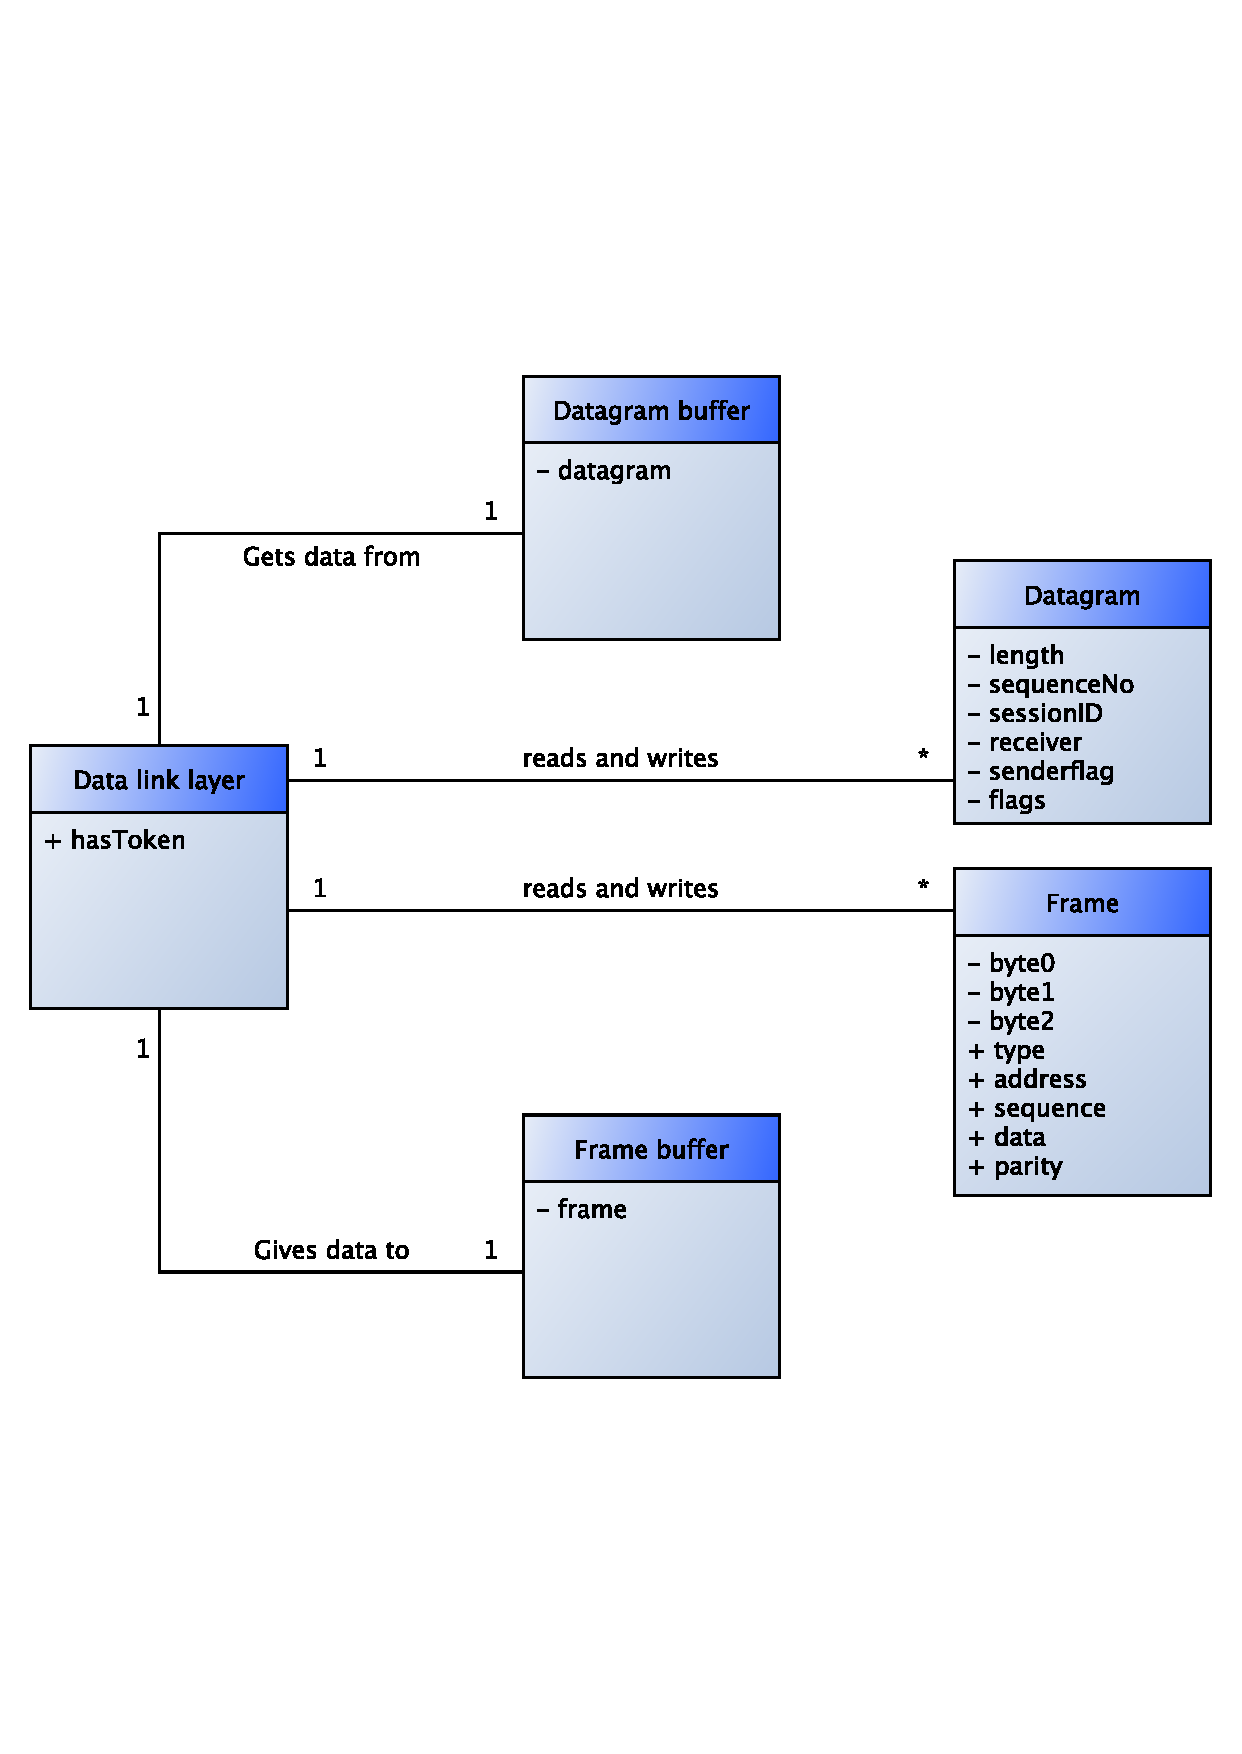
\includegraphics[scale=0.5,trim=0 0 0 0]{dll_class_diagram.pdf}
%	\caption{Class diagram for data link layer (incomplete)}
%	\label{fig:class_diag_for_datalink}	
%	\end{center}
%\end{figure}

The methods of the classes are developed to realize the flowchart of the data
link layer. Decisions on whether to implement a method in one class or another
is done using the expert pattern.

%\begin{figure}[htb]
%	\begin{center}
%	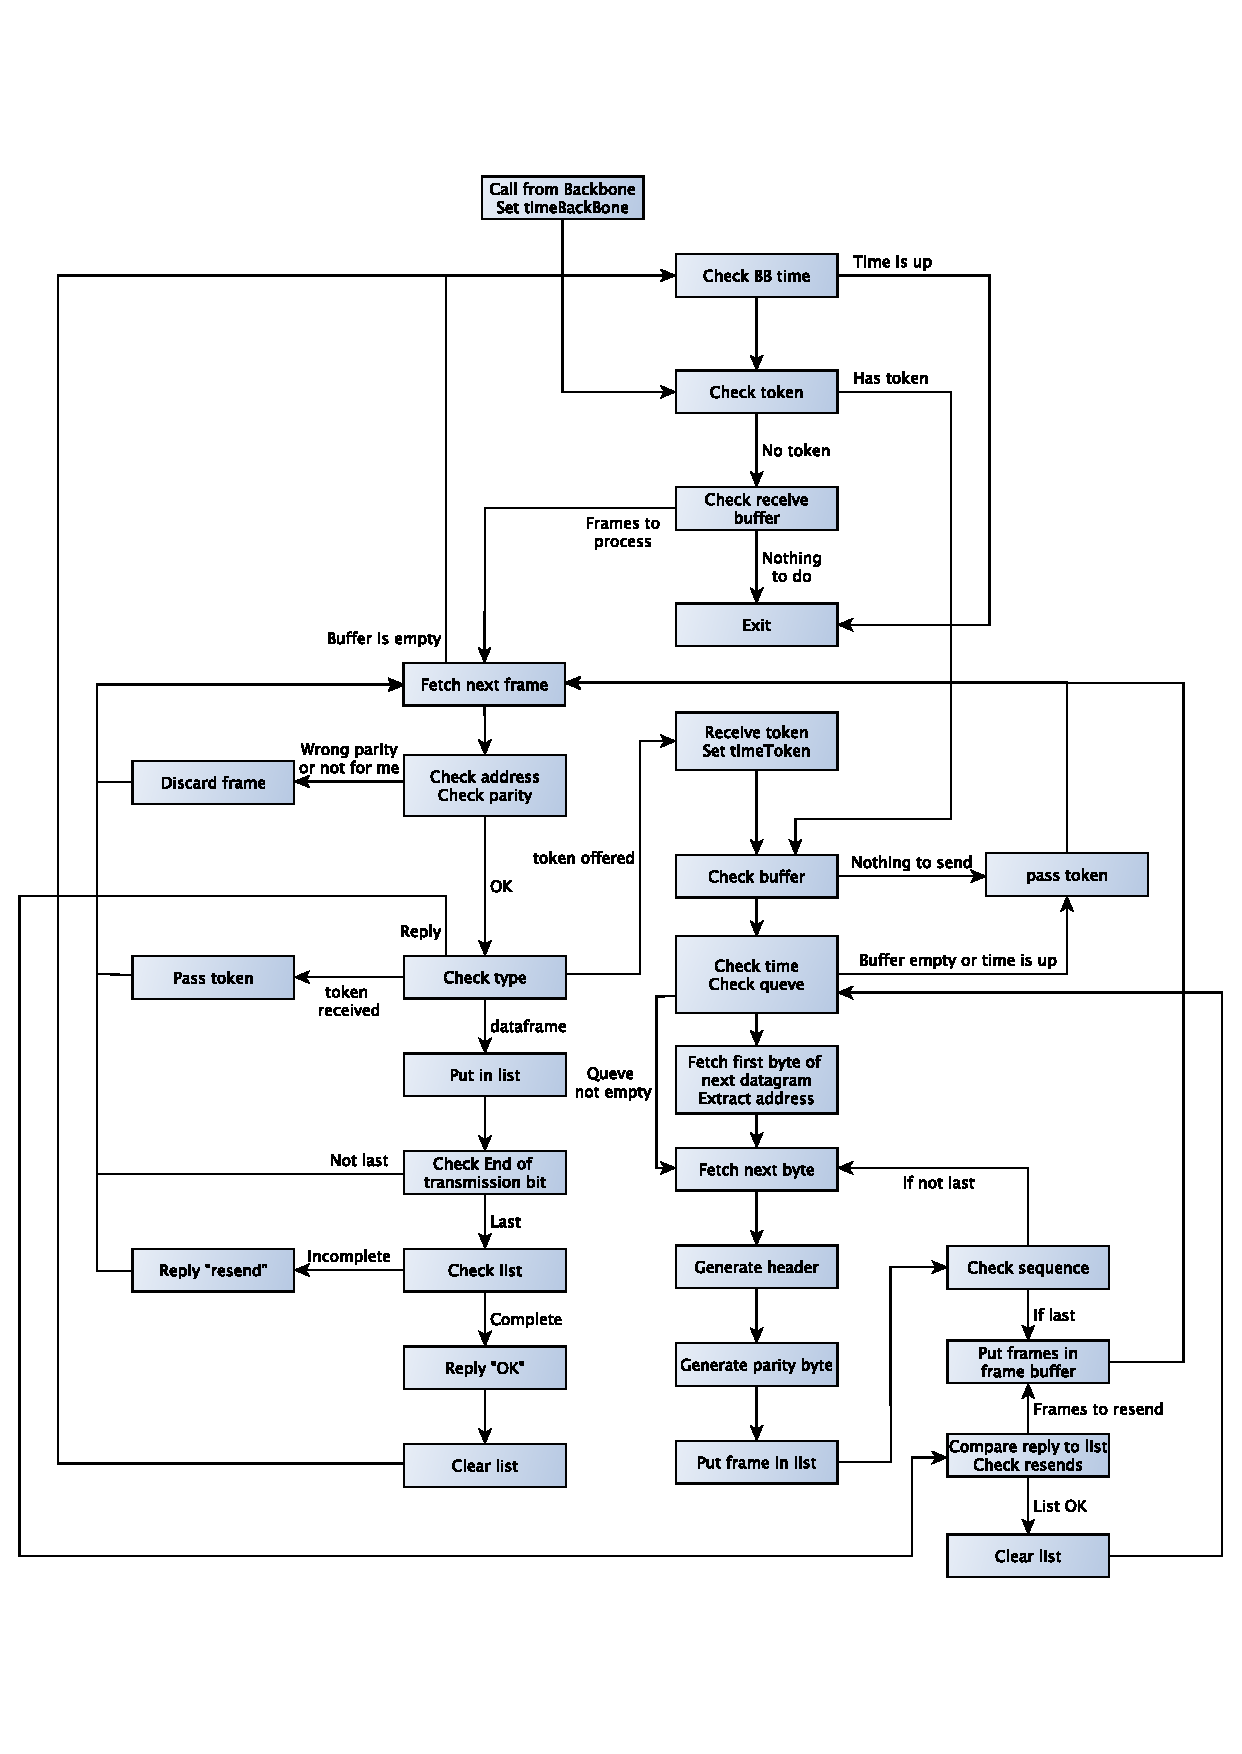
\includegraphics[scale=0.5,trim=0 0 0 0]{dll_flowchart.pdf}
%	\caption{Flowchart for data link layer}
%	\label{fig:flowchart_for_datalink}	
%	\end{center}
%\end{figure}